\chapter{Appendix}
\label{chap:appendix_reg}

\section{Word Cloud Faux Positifs}
\begin{figure}[h]
    \centering
    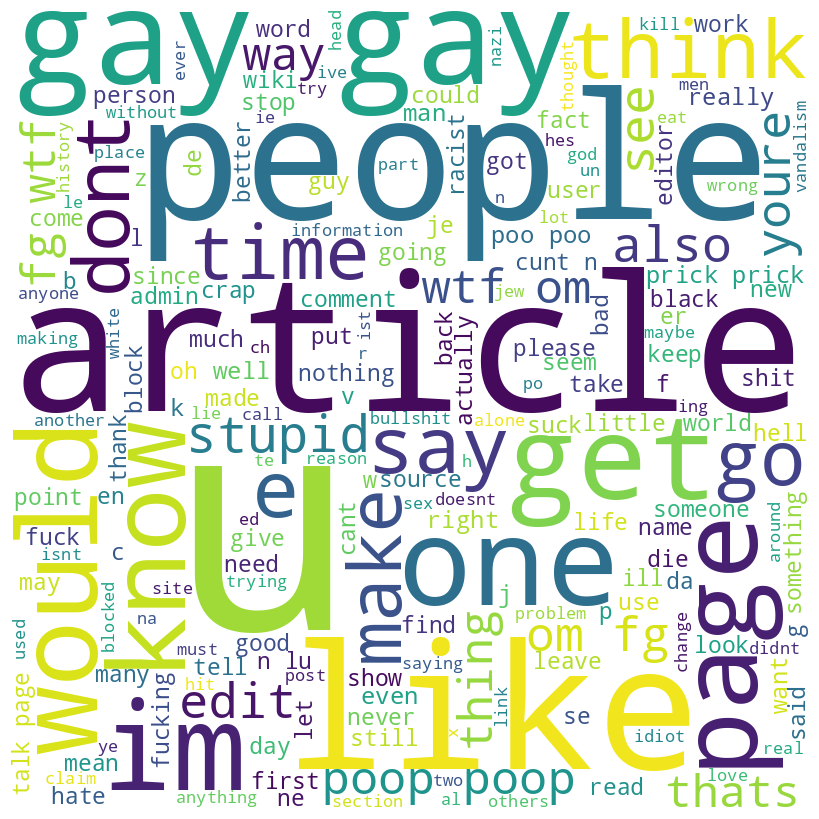
\includegraphics[width=0.4\textwidth]{figures/word-cloud-reg-tf-fp.png}
    \caption{Word Cloud Faux Positifs – Régression Logisitique TF-IDF Optimisé, sur le jeu de test. Prétraitement: BPE Tokenizer 2}
\end{figure}

\begin{figure}[h]
    \centering
    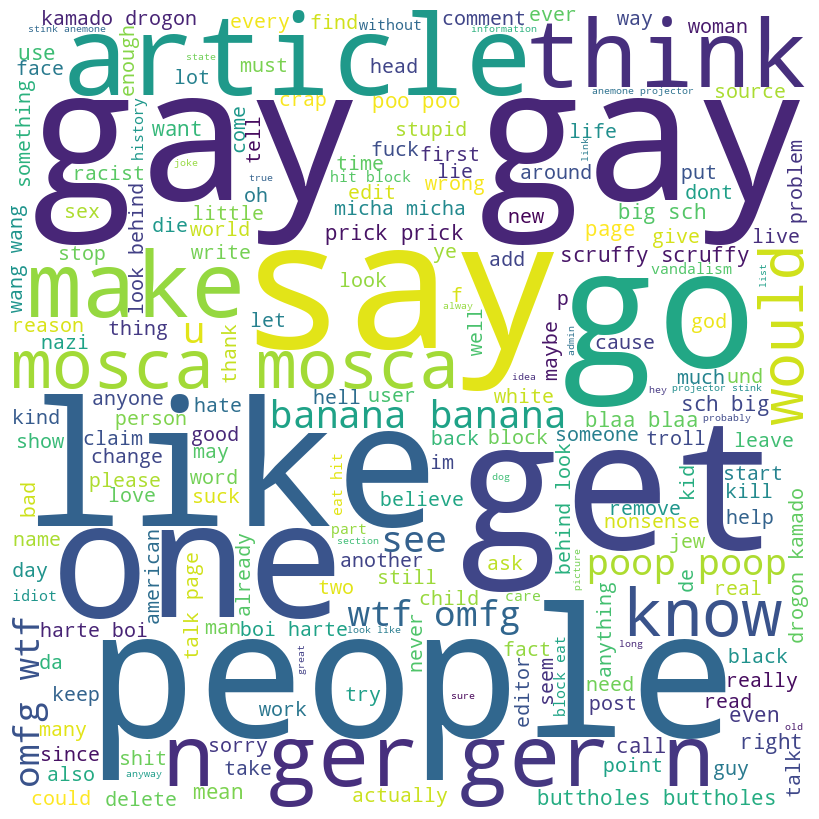
\includegraphics[width=0.4\textwidth]{figures/word-cloud-reg-w2v-fp.png}
    \caption{Word Cloud Faux Positifs – Régression Logisitique TF-IDF Optimisé, sur le jeu de test. Prétraitement: Word Tokenizer 1}
\end{figure}

\newpage
\section{Word Cloud Faux Négatifs}
\begin{figure}[h]
    \centering
    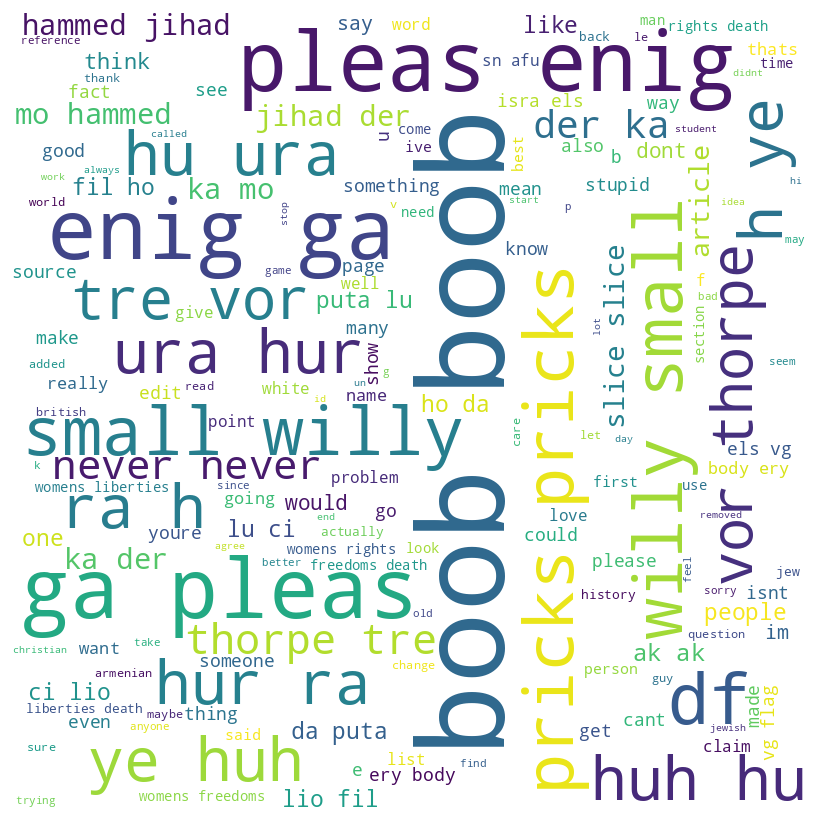
\includegraphics[width=0.4\textwidth]{figures/word-cloud-reg-tf-fn.png}
    \caption{Word Cloud Faux Négatifs – Régression Logisitique TF-IDF Optimisé, sur le jeu de test. Prétraitement: BPE Tokenizer 2}
\end{figure}


\begin{figure}[h]
    \centering
    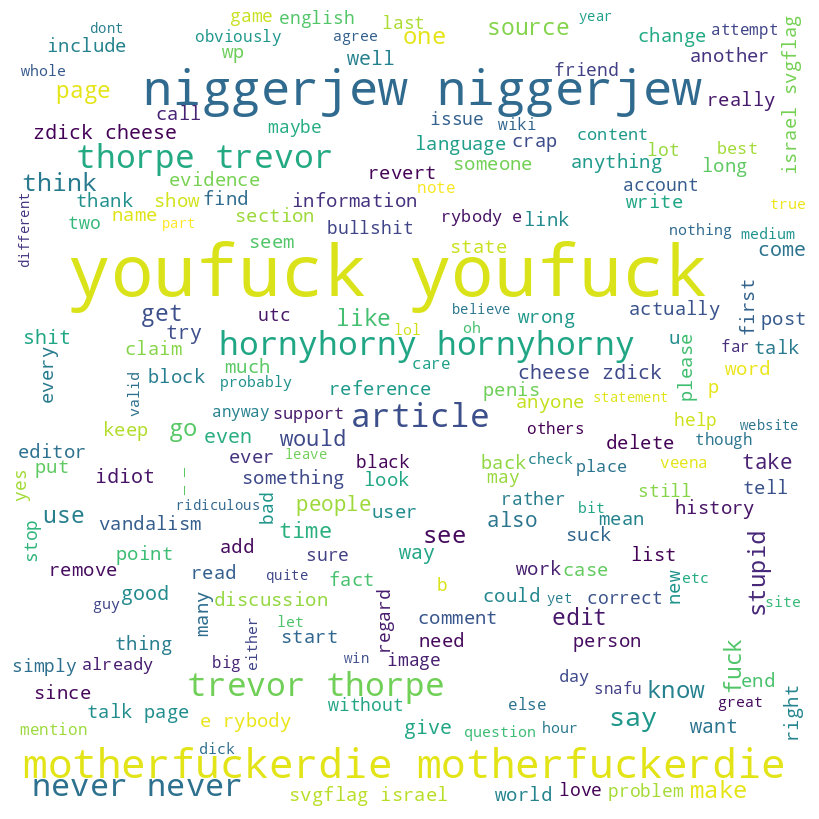
\includegraphics[width=0.4\textwidth]{figures/word-cloud-reg-w2v-fn.png}
    \caption{Word Cloud Faux Négatifs – Régression Logisitique Word2Vec Optimisé , sur le jeu de test. Prétraitement:  Word Tokenizer 1}
\end{figure}

\newpage

\section{Shap Values}
\begin{figure}[h]
    \centering
    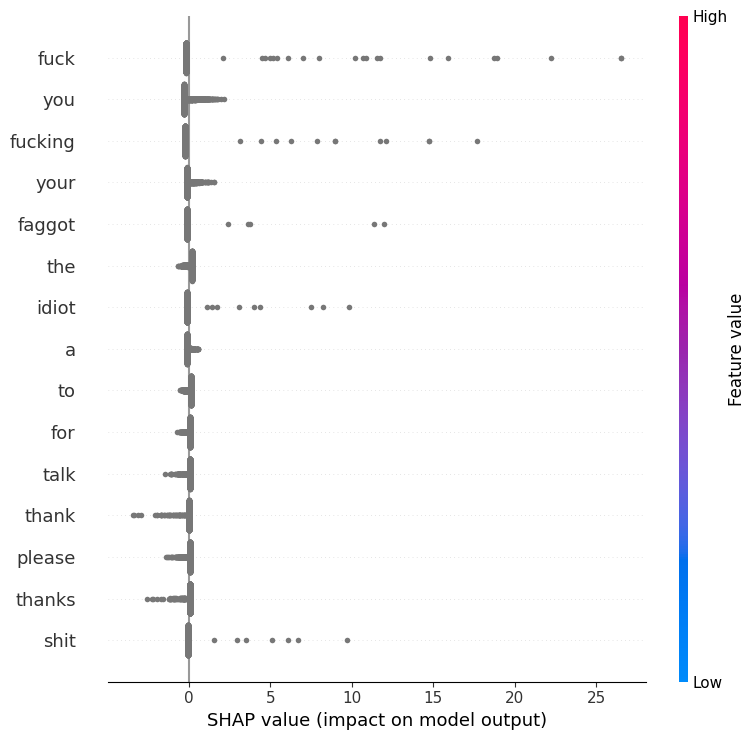
\includegraphics[width=0.9\textwidth]{figures/reg-tf-shap.png}
    \caption{Shap Values – Régression Logisitique TF-IDF Optimisé, sur le jeu de test. Prétraitement: BPE Tokenizer 2}
\end{figure}